\chapter{Développement d'un système de \textit{plugins} entrées/sorties}

\section{Définition de la mission}
\subsection{Contexte}
Dès le début du développement de Vahana VR, la question des entrées et des sorties
du logiciel s'était posée. En effet, Studio étant un logiciel de montage de vidéos
360, ses seules entrées sont des fichiers vidéos, issus des caméras de la monture. De même, la seule sortie
est le fichier vidéo 360, comme présenté dans la section \cf{exportation}.\\
Ce qui est ici appelé \emph{entrées} sont les données envoyées au programme, quand
les \emph{sorties} sont les données émises par ce programme en retour.\\
Pour permettre la vidéo 360 en direct, Vahana VR, contrairement à Studio, s'affranchit des fichiers
vidéos importés et propose de capturer directement les images des caméras, via
des cartes d'acquisitions branchées sur la machine utilisée. De même, Vahana VR peut émettre 
plusieurs fluxs en sortie permettant, par exemple, le \textit{streaming} RTMP ou la réémission vers
une carte d'acquisition SDI ou HDMI, en plus de l'export de la vidéo 360 sur le disque dur.\\
\begin{figure}
  \centering
  \setlength{\unitlength}{8mm}
  \begin{picture}(16,5)
    \linethickness{0.3mm}
    \thicklines
    \put(4,0.5){\small Entrées}
    \put(4,4.2){\vector(2,-1){2}} \put(2.2,4.2){$1$ audio }
    \put(4,3){\vector(2,0){2}}    \put(2,2.3){$n$ vidéos}
    \put(4,1.8){\vector(2,1){2}}  \put(4.1,2.2){$\Shortstack{. . . .}$}
    \put(7,0.5){\small Stitch 360}
    \put(6,2){\framebox(4,2){\large Vahana VR}}
    \put(11,0.5){\small Sorties}
    \put(10,3){\vector(3,2){2}}  \put(12.25,4.2){HDMI}
    \put(10,3){\vector(4,1){2}}  \put(12.25,3.4){SDI}
    \put(10,3){\vector(4,-1){2}} \put(12.25,2.4){RTMP}
    \put(10,3){\vector(3,-2){2}} \put(12.25,1.6){Disque dur}
  \end{picture}
  \caption{Schéma des entrées/sorties de Vahana VR}
\end{figure}

\subsection{Problématique}
Dès lors, Vahana VR étant destiné à des sociétés de production, il doit
être compatible avec un maximum de standards, caméras et cartes d'acquisitions vidéos
pour être facilement adopté. Cependant, tout matériel informatique requérant des pilotes
\footnote{Programme permettant au système d'exploitation d'interagir avec le matériel couvert par ce pilote\cite{pilote-informatique}.}
, et, les besoins des clients en entrées/sorties n'étant pas les mêmes, il n'était
alors pas possible de concevoir un logiciel monolithique contenant tous les programmes 
d'entrées/sorties supportés~: l'installation de Vahana VR aurait requis au client 
une installation de l'ensemble des pilotes.\\
De plus, un client pourrait souhaiter utiliser du matériel entrée/sortie encore
non supporté. Il serait intéressant qu'il puisse réaliser son propre développement
dans l'écosystème de Vahana VR; ainsi le logiciel pourrait devenir virtuellement
compatible avec n'importe quel standard, caméra ou carte d'acquisition.\\
Il fallait donc développer un système assurant à la fois la compatibilité
entre Vahana VR et ces matériels, et intégrant les contraintes exposées.\\

\subsection{Objectifs}
Au début de ce stage, une solution avait déjà été esquissée et était déjà en partie
mise à l'\oe uvre. Cependant un certain travail de développement était encore nécessaire.\\
\newline
Les objectifs retenus pour cette mission ont donc été~:
\begin{itemize}
  \item Développer les entrées HDMI\footnote{\textit{High Definition Multimedia Interface}, 
  norme de diffusion audio/vidéo numérique\cite{hdmi}.} et SDI\footnote{\textit{Serial Digital Interface}, 
  protocole de diffusion vidéo numérique\cite{sdi}.}.
  \item Développer les sorties HDMI et SDI.
  \item Développer des entrées/sorties Ethernet et PCIe\footnote{\textit{PCI Express}, standard
  de connexion de cartes d'extension sur la carte mère d'un ordinateur\cite{pci-express}.}
  spécifiques, à la demande d'un client.
  \item Déployer l'ensemble des \textit{plugins} sur un dépôt séparé.
  \item Documenter et vérifier la bonne intégration des \textit{plugins} dans Vahana VR.
\end{itemize}

\begin{figure}
  \centering
  \begin{minipage}{0.2\textwidth}
    \centering
    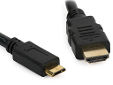
\includegraphics[width=3cm]{images/hdmi-cable.jpg}
    \captionof{subfigure}{HDMI}
  \end{minipage}%
  \hspace{0.03\textwidth}
  \begin{minipage}{0.2\textwidth}
    \centering
    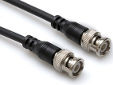
\includegraphics[width=3cm]{images/sdi-cable.jpg}
    \captionof{subfigure}{SDI}
  \end{minipage}%
  \hspace{0.03\textwidth}
  \begin{minipage}{0.2\textwidth}
    \centering
    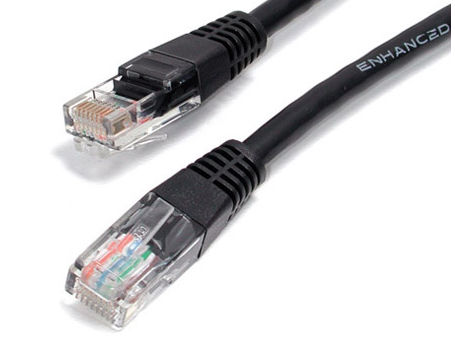
\includegraphics[width=3cm]{images/ethernet-cable.jpg}
    \captionof{subfigure}{Ethernet}
  \end{minipage}%
  \hspace{0.03\textwidth}
  \begin{minipage}{0.2\textwidth}
    \centering
    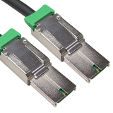
\includegraphics[width=3cm]{images/pcie-cable.jpg}
    \captionof{subfigure}{PCIe}
  \end{minipage}
  \caption{Illustration des différents connecteurs utilisés par Vahana VR}
\end{figure}


\section{Réalisation}
\subsection{Architecture de la solution}
Il s'agissait tout d'abord de saisir le concept de la Programmation Orientée Composant, et la manière
dont il est appliqué pour Vahana VR.
Cette approche propose d'utiliser différents \emph{composants}, c'est-à-dire des briques logicielles
qui peuvent interagir entre elles. Tout comme les dépendances\footnote{Présentées dans 
la section \cf{integration-dependances-player}.}, un composant va fournir un ensemble
de fonctions, présentes dans des bibliothèques (fichiers .dll sous Windows). Elles sont
déclarées dans les \textit{headers} qui accompagnent ces bibliothèques, afin de 
pouvoir être utilisées par les autres composants.\cite{poc}\\
Ici, on parle un peu plus spécifiquement de \textit{plugins} et de \emph{programme client}.
Les \textit{plugins} peuvent être chargées et utilisées par un programme client, 
ici Vahana VR. Leurs fonctions sont donc regroupées en des modules externes
au logiciel qui peut y faire appel si besoin, ou non. Leurs interfaces sont, cette
fois, définies dans le logiciel.\cite{plugin}\\
Un \textit{plugin} est donc utilisé indirectement via ses interfaces et \emph{dynamiquement}.
Car c'est à son lancement que le programme charge les \textit{plugins}~:
il va rechercher ceux implémentant les interfaces attendues. En effet,
le code de la bibliothèque est inconnu car compilé, seul sont connues les fonctions 
attendues du \textit{plugin}.\\
\newline
Un exemple de \textit{plugins} sont typiquement les extensions d'un navigateur web. Ces composants
ont été écrits pour le navigateur, en répondant à une interface attendue par ce logiciel,
et peuvent être activés ou désactivés à volonté par l'utilisateur.\\
L'intérêt d'une telle approche est qu'elle permet d'introduire de la modularité dans 
l'architecture du projet, les \textit{plugins} pouvant être développés séparément du logiciel
client. Et surtout, ils peuvent être distribués séparément du logiciel ou être remplacés
au besoin sans remplacer tout le logiciel. Cela peut présenter une difficulté d'analyse~:
quoi externaliser dans des plugins ? et sous quelles interfaces ? Car si les interfaces
changent, le composant doit obligatoirement être remplacé et mis-à-jour, brisant la compatibilité
des anciennes versions.\cite{poc}\\ 
\newline
Concrètement, Vahana VR définit trois interfaces à implémenter pour les \textit{plugins}~:
\begin{itemize}
  \item Une interface pour créer une entrée.
  \item Une interface pour créer une sortie.
  \item Une interface \textit{discovery} dont le rôle est d'indiquer les possibilités
    de créations entrées/sorties.
\end{itemize}
Le diagramme de classes UML de la figure~\ref{uml-interfaces} les détaille.\\
\begin{figure}
  \centering
  \caption{Diagramme de classes des interfaces}
  \label{uml-interfaces}
\end{figure}
Ainsi, lors de son exécution, Vahana VR va chercher les bibliothèques présentes dans le dossier
\shellinline{plugins} à sa racine et va charger les \textit{plugins} implémentant
au moins un de ces interfaces. Une fois chargés, le logiciel possède désormais une collection d'entrées
ou de sorties potentielles. En fonction de données renvoyée par les \textit{discovery},
l'utilisateur peut demander, dans l'interface de Vahana VR, de 
créer une nouvelle entrée -- ou sortie -- pour \textit{plugin}. Et via les
interface implémentées par le \textit{plugin}, le logiciel va pouvoir faire exécuter le code
de création de l'entrée -- ou sortie -- du \textit{plugin}.\\

\subsection{Conception des \textit{plugins}}
Cinq \textit{plugins} furent écrits et maintenus pour répondre aux besoins. Ils s'appuient 
tous sur du matériel, comme des caméras ou des cartes d'acquisitions, conçu par 
des entreprise externes à VideoStitch.
L'approche retenue a donc été de créer un nouveau \textit{plugin} par constructeur~:
\begin{itemize}
  \item Entrée/sortie SDI et HDMI avec les cartes d'acquisition DeckLink
  \footnote{\url{https://www.blackmagicdesign.com/fr/products/decklink/models}}.
  \item Entrée HDMI avec les cartes d'acquisition Yuan
  \footnote{\url{http://www.yuan.com.tw/en/products/capture/capture_mod.htm}}.
  \item Entrée HDMI avec les cartes d'acquisition Magewell
  \footnote{\url{http://www.magewell.com/hardware?lang=en}}.
  \item Entrée PCIe avec les caméras xiB de Ximea
  \footnote{\url{http://www.ximea.com/en/products/application-specific-oem-and-custom-cameras/pci-express-high-speed-cameras}}.
  \item Entrée Ethernet GigE\footnote{Standard pour les caméras industrielle utilisant 
  la transmission par Ethernet\cite{gige}.} avec les caméras Genie TS de Teledyne Dalsa\footnote{\url{http://www.teledynedalsa.com/imaging/products/cameras/area-scan/genie-ts/}}.
\end{itemize}
\ \\
Leurs développements respectifs ont suivis les même étapes~:

\subsubsection{Prise en main}
Tout d'abord, il s'agissait d'installer la caméra ou la carte d'acquisition sur la 
machine de développement et de la mettre en fonctionnement. Le constructeur va fournir
deux ressources~: le pilote pour que le système puisse utiliser le matériel, et un
SDK pour qu'un développeur puisse écrire une application utilisant ce matériel.
Ce SDK est donc une dépendance du plugin~: ses \textit{headers} et bibliothèques
ont été ajoutés au dépendances sur le dépôt VideoStitch-deps.\\
\begin{figure}
  \centering
  \setlength{\unitlength}{4mm}
  \begin{picture}(10,14)
    \linethickness{0.3mm}
    \thicklines
    \put(2,12){\framebox(6,2){Vahana VR}}       \put(4,12){\vector(0,-1){1}} \put(6,11){\vector(0,1){1}}
    \put(2,9){\framebox(6,2){\textit{Plugin}}}  \put(4,9){\vector(0,-1){1}}  \put(6,8){\vector(0,1){1}}
    \put(0,6){\framebox(10,2){SDK constructeur}} \put(4,6){\vector(0,-1){1}}  \put(6,5){\vector(0,1){1}}
    \put(2,3){\framebox(6,2){Driver}}           \put(4,3){\vector(0,-1){1}}  \put(6,2){\vector(0,1){1}}
    \put(2,0){\framebox(6,2){Matériel}}
  \end{picture}
  \caption{Schéma des interactions de Vahana VR au matériel d'entrées/sorties}
  \label{entree-sortie-schema}
\end{figure}
La figure~\ref{entree-sortie-schema} résume les interactions de Vahana VR au matériel d'entrée/sortie~:
les \textit{plugins} correspondent au patron de conception\footnote{Ou \textit{design pattern},
qui est une bonne pratique de conception logicielle.} \emph{adaptateur}, c'est-à-dire qu'ils convertissent les interfaces
et le fonctionnement du SDK du constructeur sous d'autres interfaces, celles attendues
par le programme client, Vahana VR\cite{adapter-design-pattern}.

\subsubsection{Implémentations}
Ces interfaces attendues sont définies dans Vahana, et développer un \textit{plugin} consiste
à en réaliser les implémentations~: ce fut la seconde partie du développement.\\
Tous les \textit{plugins} développés implémentent l'interface \cppinline{Input}
et ses fonctions~:
\begin{itemize}
  \item \cppinline{ing handle(const Config* parameters)} : indique si le
  plugin peut prendre en charge ces paramètres pour créer l'entrée.
  \item \cppinline{Input* create(const Config* parameters)} : appellée si \cppinline{handle}
  a réussi, cette fonction tente la création de l'entrée avec les paramètres donnés
  et renvoie un pointeur sur l'objet \cppinline{Input} créé si cela a réussi, sinon
  un pointeur nul.
  \item \cppinline{bool readFrame(uint32_t* frame)} : cette fonction renvoie la
  dernière image capturée par la caméra -- ou carte d'acquisition --. Elle est
  appellée autant de fois que précisé dans les paramètres de la configuration,
  généralement au moins 25 fois par seconde pour obtenir une image fluide.\\
  L'image doit être renvoyée dans le format de couleur RGBA.
\end{itemize}
L'implémentation de l'interface \cppinline{Output} est similaire à l'interface \cppinline{Input},
à la différence qu'elle envoie des images, avec la méthode \cppinline{writeFrame}, 
à l'instar de la méthode \cppinline{readFrame}.\\
\newline
La création d'un \cppinline{Input} réclame donc quelques paramètres et leurs valeurs, envoyés 
au travers de l'argument \cppinline{parameters}. Cette configuration fournie par
l'utilisateur contient, par exemple~:
\begin{itemize}
  \item Le nom du plugin cherché.
  \item Quelle caméra du plugin utiliser.
  \item La résolution désirée de la vidéo à capturer (largeur et hauteur en pixel).
  \item Le \textit{framerate}, c'est-à-dire le nombre d'images par seconde qui 
  seront capturées. C'est ce paramètre qui règle le nombre 
  d'appels par secondes que Vahana VR va faire de la fonction \cppinline{readFrame}.
  \item Le \textit{pixel format} utilisé, c'est-à-dire le format de couleur. Un 
  certain nombre d'encodages des couleurs pour un pixel existent et une sortie peut attendre un
  format bien particulier, tout comme une entrée peut retourner des images sous un
  format précis.
\end{itemize}
Cette liste est enrichie par d'autres paramètres selon chaque \textit{plugin} et 
les capacités du SDK du constructeur. Par exemple, Ximea propose des réglages
de l'objectif de la caméra.\\
\newline
L'interface \cppinline{Discovery} permet d'indiquer à Vahana VR, et par extension
à l'utilisateur, les ensembles de de paramètres et valeurs utilisables pour la
création des entrées/sorties du \textit{plugin}. 
L'implémentation de cette interface s'effectue avec quelques fonctions~:
\begin{itemize}
  \item \cppinline{std::string name()}~: indique le nom du plugin, qui sera utilisé
  dans par les paramètres de configuration.
  \item \cppinline{std::vector<Device> devices()}~: indique la liste des entrées/sorties
  disponibles~: pour les cartes d'acquision cela correspond à l'ensemble des ports
  entrées/sorties présents sur la carte; quand aux caméras, seules celles branchées apparraîtront. 
  Un \cppinline{Device} est simplement le numéro de la caméra, ou du port, ainsi
  que son type~: entrée, sortie, ou les deux.
  \item \cppinline{std::vector<DisplayMode> supportedDisplayModes(const Device& device)}~:
  retourne l'ensemble des couples résolution-\textit{framerate} supportés par le \textit{device}.
  \item \cppinline{std::vector<PixelFormats> supportedPixelFormat(const Device& device)}~:
  retourne l'ensemble des formats de couleur supportés par le \textit{device}.\end{itemize}
\ \\
La documentation accompagnant les SDK est ensuite lue, tout comme les programmes
examples fournis, pour comprendre les possiblités offertes, définir les différents
paramètres qui seront utilisés, et, enfin, implémenter les fonctions des interfaces.\\
Un résumé global de ces implémentations peut être décrit, les approches des différents SDK restant globalement
les mêmes.
Par exemple, voici l'implémentation des méthodes \shellinline{create(const Config* parameters)} 
et \shellinline{devices()}, dont les fonctionnements sont assez similaires~:
\begin{enumerate}
  \item Tout d'abord, une initialisation du SDK du constructeur est réalisée. Si
  elle échoue, le driver n'est alors pas installé.
  \item Seulement pour \shellinline{create} sont récupéré l'ensemble des paramètres
  de la configuration et la validité de leurs valeurs est testée.
  \item Une itération est réalisée sur tous les \textit{devices} disponibles.\\
  \shellinline{create} va sélectionner celui précisé dans les paramètres, quand \shellinline{devices}
  va tous les garder en mémoire.
  \item Un pointeur\footnote{Ou encore appelé \textit{handle} dans les SDK utilisant 
  le système COM de Microsoft.} est récupéré sur chaque \textit{device} sélectionné
  à l'étape précédente.
  \item Grace à ce pointeur, le \textit{device} est configuré~: selon les paramètres
  pour \shellinline{create} ou afin de préparer la détection des paramètres supportés pour
  \shellinline{devices}.
  \item Seulement pour \shellinline{create} est lancée la capture vidéo.
  \item Enfin la méthode se termine et retourne un pointeur sur l'objet implémentant
  l'interface \shellinline{Input} pour \shellinline{create}; ou la liste des \shellinline{devices}
  pour la fonction \shellinline{devices}.
\end{enumerate}
Si une de ses étape échoue, la méthode s'arrête à son tour et écrit un message d'erreur
qui pourra être récupéré et affiché par Vahana VR à l'utilisateur.\\
\newline
De même, la fonction \shellinline{readFrame} consiste toujours en deux étapes~:
\begin{enumerate}
  \item Lire la dernière image capturée par l'entrée.
  \item Transformer l'image du format de couleurs de capture vers le format de couleurs
  RGBA. En effet, pour optimiser les algorithmes, les applications VideoStitch
  ne travaillent qu'avec ce format. Ainsi un certain nombre de fonctions, utilisant
  CUDA\footnote{Voir la section \cf{videostitch-sdk-section}.}, sont disponibles pour opérer ces transformations vers le RGBA.
  La méthode appelle simplement la fonction nécessaire et en copie le résultat dans le
  tampon \cppinline{uint32_t* frame} pour Vahana VR.
\end{enumerate}

\subsection{Quelques problèmes et solutions spécifiques}
Chaque \textit{plugin} s'appuyant sur un SDK d'un constructeur différent, un certain nombre
de problèmes furent rencontrés pour réaliser l'implémentation totale des interfaces.
Quelques difficultés et leurs solutions sont notables.

\subsubsection{Fonctions de rappel}
La fonction \shellinline{readFrame} a souvent été mise en \oe uvre par un systèmes
de fonctions de rappels~: bien souvent pour récupérer les images, il fallait passer au 
SDK lors de la configuration de l'entrée un pointeur sur une fonction\cite{fonction-de-rappel}.
Ainsi à chaque image capturée par la caméra ou le port, cette fonction de rappel sera appellée
par le SDK avec le contenu de l'image en argument. Ce contenu est donc écrit dans
une variable du plugin qui sera lue par la méthode \shellinline{readFrame}.\\
Dès lors, il peut se créer un problème de synchronisation entre ces deux fonctions.
La ressource partagée doit être protégée d'une double utilisation~: une exclusion
mutuelle\cite{exclusion-mutuelle} a été mise en place. De plus, la ressource ne doit 
être écrite qu'une fois qu'elle a été lue~: les deux fonctions ont donc été placées 
dans des threads séparés et une condition variable a été utilisée. C'est une primite
de synchronisation C++ qui permet de bloquer deux threads jusqu'à l'un reçoive une
notification de l'autre\cite{condition-variable}~: que la variable a été lue pour
la fonction de rappel, et que la variable a été écrite pour la fonction \shellinline{readFrame}.

\subsubsection{Partage des ressources Yuan}

\subsubsection{Augmentation des interfaces DeckLink}

\subsubsection{Lecture des images Ximea}


\section{Déploiement}
\subsection{Création du dépôt VideoStitch-IO}
Les \textit{plugins} étaient à l'origine développés dans le dépôt VideoStitch-apps. Il faisait
cependant plus sens qu'ils soient déplacés dans un dépôt distinct, car étant relativement indépendant
de Vahana VR. Cette opération nécessitait, comme dans la section \cf{integration-apps}, un déplacement du dossier
de développement et de l'historique des modifications. La technique présentée en annexe~
\ref{deplacer-historique-depots} (p.\pageref{deplacer-historique-depots}) fut de
nouveau utilisée avec succès, déplaçant le contenu du dossier \mintinline{shell-session}{src/plugins/}
du dépôt VideoStitch-apps vers le dossier \mintinline{shell-session}{src/} sur le dépôt VideoStitch-IO.\\
\newline
Ce nouveau dépôt a été organisé de manière sensiblement équivalente à celui de VideoStitch-apps, 
cependant la chaîne de compilation des \textit{plugins} fut mise à jour pour prendre en compte
cette nouvelle organisation.\\
En outre, ce dépôt nécessitait, tout comme VideoStitch-apps, du VideoStitch-SDK et des dépendances
pour être compilé. Le script \mintinline{shell-session}{update.sh}\footnote{Voir la section \cf{integration-apps}.}
fut alors partagé, et les \textit{plugins} purent être compilés à nouveau.\\
\newline
Le Buildbot fut alors mis à jour également d'un nouveau builder prenant en charge ce dépôt.
Une liste d'étapes similaires au listing~\ref{windows-apps} (p.\pageref{windows-apps}) furent écrites pour
compiler automatiquement les \textit{plugins} et les mettre à disposition sur une page de 
téléchargement interne.\\
Le script \mintinline{shell-session}{update.sh} a alors été augmenté pour télécharger
la dernière version des \textit{plugins} et les copier dans la copie du dépôt VideoStitch-apps
du développeur appelant le script. Les \textit{plugins} ont été déplacés sur un autre dépôt
mais sont toujours nécessaires pour générer utiliser Vahana VR avec toutes ses
capacités.\\
Enfin, les \textit{plugins} DeckLink, Magewell et Yuan furent ajoutés à l'installateur de Vahana VR, 
permettant de couvrir les besoins usuels du logiciel et les caméras les plus répandues
sur le marché~: les entrées/sorties SDI et HDMI.

\subsection{Documentation}
Une documentation fut écrite pour chaque \textit{plugin}, décrivant
essentiellement leur usage aux développeurs et aux utilisateurs avancés~: l'interface
de Vahana VR devrait normalement suffire à créer les entrées et sorties. Ces documentations
reviennent sur l'installation des drivers, quel SDK et quelle version a été utilisée,
et quels paramètres, avec leurs valeurs possibles, sont utilisés par le plugin.\\
Ces documentations sont toutes rappatriées et fusionnées à celle de Vahana VR 
qui est ajoutée à l'installateur.\\
\newline
En outre, une documentation générale fut écrite sur le wiki interne. Cette version revient
plus spéciquement sur chaque plugin~: quels interfaces sont implémentées, comment
et pourquoi. Un état de l'avancement et de fonctionnement de chaque plugin 
a été tenu à jour.

\subsection{Tests et \textit{QA} de l'intégration des \textit{plugins}}
En parallèle au développement des plugins, l'équipe travailla à leur intégration
dans Vahana VR grâce aux interfaces, qui étaient déjà connues. L'utilisation de plugins
se révéla particulièrement pratique~: il suffisait de remplacer les bibliothèques par de nouvelles versions pour
obtenir les nouvelles capacitées implémentées.\\
\newline
Ce développement en parallèle fut très utile, car l'équipe de développement étant 
cliente de ses plugins, de nombreux tests furent effectués pour s'assurer d'une part 
de la bonne implémentation des plugins, et d'autre part de leur bonne intégration dans Vahana VR.
Combiné à l'utilisation des pratiques agiles, les tickets de cette mission ont vu
un certains nombre d'aller retour entre leur \textit{QA} par l'équipe et leur développement,
que ce soit pour des bogues ou des cas d'usages non prévus.\\
Pour achever cet audit qualité, de nombreuses démonstrations complète ont été faites
sur des machines de démonstration vierge d'environnement de développement, et quelques
clients, dits \textit{early adopter}, ont pu avoir accès aux plugins, alors encore en
développement, notamment pour les utiliser sur des caméras, cartes d'acquisition ou
écrans (pour récupérer les sorties) n'ayant pas été testés en interne. Pour exemple,
il est arrivé à deux reprise d'organiser une journée de travail en conversation
avec un client pour obtenir une version fonctionnelle à ses besoin. D'après ses
retours, je corrigeais le plugin, et le renvoyais compilé afin qu'il le remplace
simplement dans son dossier d'installation et le teste à nouveau.\\
Par ces pratiques, les plugins ont au final gagné en qualité et stabilité.\\
\newline
Enfin, les deux plugins Teledyne Dalsa et Ximea ont fait l'objet de démonstrations
vidéo dans Vahana VR pour le client, pour montrer les fonctionnalités et performances
du logiciel et ses capacités d'intégration de nouvelles caméras. La dernière semaine
du stage eut lieu une démonstration en direct en présence du client de l'utilisation
des caméras Ximea dans Vahana VR.

\section{Bilan et suite}
Cette mission a permis d'apporter, sous forme de modules utilisables par Vahana VR,
un certain nombre de capacités entrées/sorties au logiciel principalement sur 
des standards vidéos comme le SDI et le HDMI. D'autres standards ont pu être supportés
tout aussi facilement pour le compte d'un client.\\
L'intégration de ces plugins a pu être réalisée en parallèle de cette mission, ce
qui a été un gain de rapidité de développement mais aussi un gain de stabilité important~:
l'architecture modulaire permet de n'utiliser que les plugins désirés, sous la version
voulue.\\
C'est également pourquoi ces plugins ont été externalisés dans un dépôt différent~:
leur cycle de développement est indépendant du logiciel. En outre, Vahana VR étant
client de ces composants, des tests importants et utiles de qualité ont pu être menés
sur ces plugins. Une grande partie du succès de ce logiciel qui sortira prochainnement
tiendra à sa capacité à supporter de nombreuses entrées/sorties vidéo.\\
\newline
Il reste cependant du travail a effectuer~: les interfaces entrées/sorties devraient
être augmentées pour prendre en charge l'audio, et l'interface \textit{discovery}
devrait intégrer une détection de signal des paramètres actuellement configurés
sur les caméras branchées en entrée ou sur les écrans en sorties.\\
Par ailleurs l'architecture de cette solution est une grande qualité, car de nouveaux
plugins pourront être développés très facilement~: il pourrait être très intéressant
d'ouvrir les sources de ce dépôt aux clients afin qu'ils puissent développer le
support de leur propre matériel dans l'ecosystème de Vahana VR. Une interface de programmation
\footnote{Ou API pour \textit{Application Programming Interface}, est une interface
par laquelle un logiciel offre des services à un autre logiciel\cite{interface-programmation}.} 
pourrait être même plus généralement développée pour l'intégralité du logiciel,
pour, à l'instar de toutes les grandes entreprises du web\cite{interface-programmation}, 
développer de nouveaux marchés et tisser de nombreuses interactions avec d'autres
écosystèmes\cite{valeur-api}\cite{value-apis}, chacun devenant composant d'un système
d'innovation et de croissance inter-logiciels.

